\section{Anotações importantes da observação}

\subsection{Os primeiros vídeos}

O primeiro vídeo data de 09/MAI/2014, link \url{https://www.youtube.com/watch?v=8xyller_i5w}, ela com 12 anos ensinando a fazer caixas de doces decoradas, como denuncia a tag \#DIY\footnote{acrônimo de Do it Yourself, faça você mesmo} de Faça Você Mesmo. O vídeo é curto e demonstra que a menina possui desenvoltura e a mesma não se intimida pela câmera. A desenvoltura com que a mesma faz a caixa de doce sugere que ela já lida com trabalhos manuais com muita frequência.

Seguem-se outros vídeos com mesma temática de faça você mesmo, além de experimentação de guloseimas. Num deles faz um react\footnote{react é o termo usados pelos youtubers para reagir a algum fato pela primeira vez} de um unboxing de guloseimas comprados no bairro oriental da Liberdade em SP (\url{https://www.youtube.com/watch?v=qrBjcxeDKJE}). Ela dedica vários vídeos de doces orientais, incluindo os gravados com a mãe.

Nítido notar que a Zabetta é uma menina no final da puberdade, com feições infantis encontrados em qualquer menina da sua idade.

Ela mostra que já tem um time de coração, o Palmeiras, o que demonstra no vídeo \url{https://www.youtube.com/watch?v=W_LVN3bIKqo}, pena que não tem bastidores do pós-jogo para verificar as reações.

Durante um bom tempo ela se dedicou a vídeos de faça você mesma, muito inspirado nos trabalhos da mãe, Ane Macarini, que se considera Cake Design (Designer de Bolos). Inclusive fica evidente que a mãe incentiva e participa do conteúdo a ser produzido.

Como toda menina, ela sonha em ser atriz, inclusive fez teste de elenco com decoreba de texto no SBT\footnote{SBT - Sistema Brasileiro de Televisão} como demonstrado no vídeo \url{https://www.youtube.com/watch?v=iAzd_bcn_3c}. O vídeo é um grande registro de tietagem tanto dela como o da mãe. A relação com a mãe é de muita proximidade.

Interessante reparar que existe aprovação e controle da mãe sobre o conteúdo colocado no YouTube, o que seria normal da idade. Como a série de vídeos com o tema Halloween.

No vídeo \url{https://www.youtube.com/watch?v=f-FUL9s_0cU} foi um compilado de perguntas e respostas, onde é evidenciado que o pet da casa, uma cachorra chamada Bella. É revelado que Zabetta é um nome de origem italiana que possui tradição na família, o que reforça que existem laços e tradições fortes. A Zabetta já fez algumas figurações, o que responde sobre a desenvoltura em frente as câmeras.

No aniversário de 13 anos, ela demonstrou seus presentes no vídeo \url{https://www.youtube.com/watch?v=nCskv33ok08} o fato curioso é ela ter ganho um cartão de crédito do tipo mesada, indicando preocupação dos pais com a educação financeira ou controle do que é gasto pela filha. O engajamento do colégio (Objetivo) com seus alunos foi mencionado na festa surpresa preparada pela mãe e as coordenadoras. A fala é desenvolta mas compatível do que se espera de vocabulário e articulação de uma criança de 13 anos. Fora uma comemoração em família no Outback no vídeo \url{https://www.youtube.com/watch?v=Fsuw8c0nYP0}.

No vídeo \url{https://www.youtube.com/watch?v=QDMu3dTOoVI} ela brinca num desafio com cereja e chantily vemos que ela é a caçula de outros 3 irmãos. Aparentemente eles são muito amorosos um com outro.

No vídeo \url{https://www.youtube.com/watch?v=z0VjIP5AUAU} ela se permite mostrar alguns erros de gravação, mostrando um pouco dela como ela realmente é. Nesse vídeo mostra a interação com produtos que ela ganhou de aniversário. Fácil notar que tirando o HD e o PowerBank indutivo, todos os demais produtos são do universo feminino, maquiagem e beleza.




\begin{figure}
    \centering
    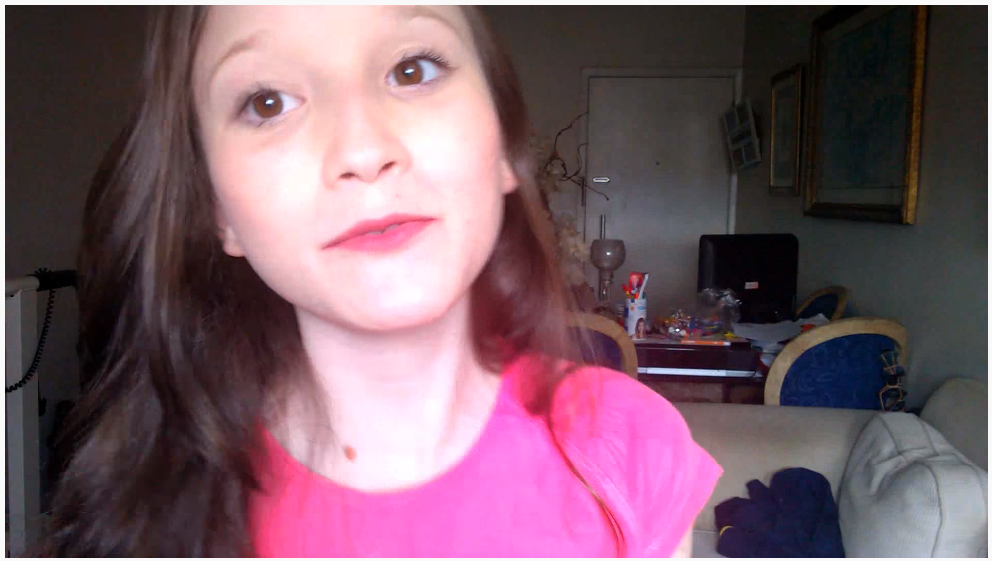
\includegraphics[width=0.7\linewidth]{fig/Zabetta-12-anos}
    \caption{vb}
    \label{fig:zabetta-13-anos}
\end{figure}


